Les diagrammes de classes participantes sont représentés dans cette 
partie. Il y en a un par cas d'utilisation.

Les accesseurs se trouvent ici dans les contrôleurs comme l'UML l'autorise. Lors de l'implémentation, ils pourraient être déplacés dans le modèle selon la solution choisie.

\section{Se connecter au bureau distribué}

\begin{figure}[H]
	\centering
	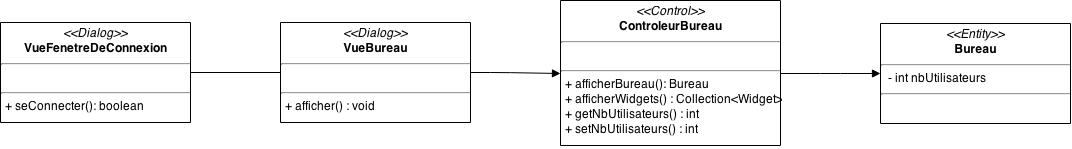
\includegraphics[scale=0.3]{diagrammes/DCP1.png}
	\caption{Diagramme de Classes Participantes, cas 1}
\end{figure}

\section{Ouvrir une fenêtre}

\begin{figure}[H]
	\centering
	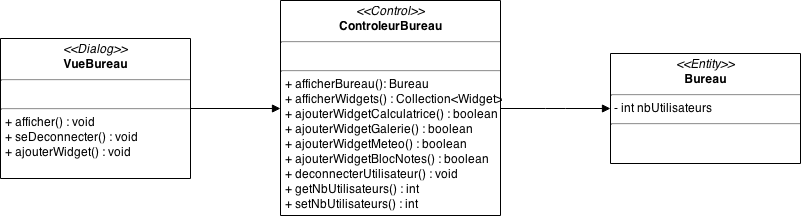
\includegraphics[scale=0.4]{diagrammes/DCP2.png}
	\caption{Diagramme de Classes Participantes, cas 2}
\end{figure}

\section{Saisir une opération}

\begin{figure}[H]
	\centering
	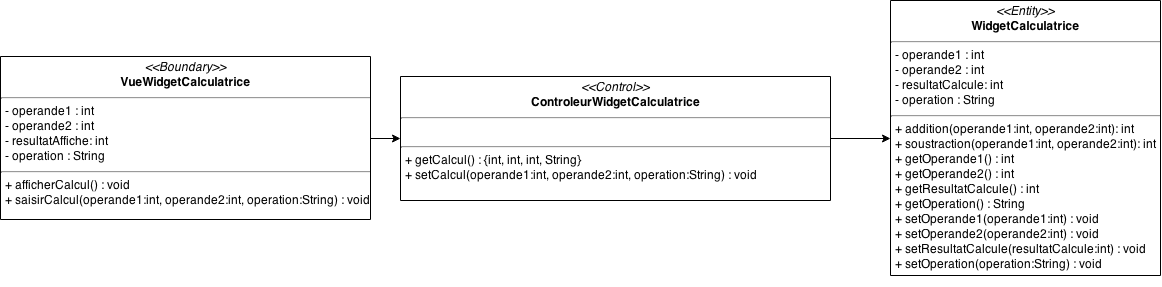
\includegraphics[scale=0.3]{diagrammes/DCP3.png}
	\caption{Diagramme de Classes Participantes, cas 3}
\end{figure}

\section{Regarder des photos}

\begin{figure}[H]
	\centering
	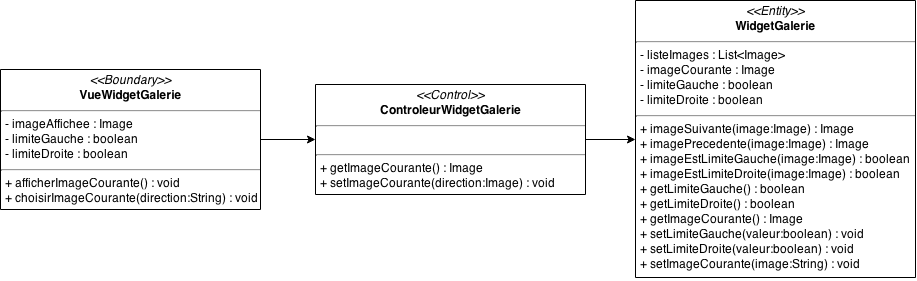
\includegraphics[scale=0.4]{diagrammes/DCP4.png}
	\caption{Diagramme de Classes Participantes, cas 4}
\end{figure}

\section{Quitter le bureau virtuel}

\begin{figure}[H]
	\centering
	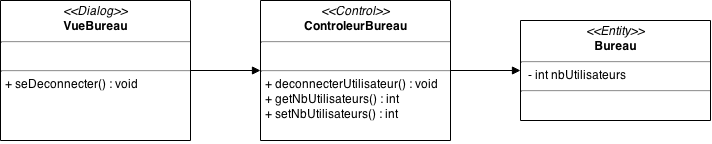
\includegraphics[scale=0.4]{diagrammes/DCP5.png}
	\caption{Diagramme de Classes Participantes, cas 5}
\end{figure}